\documentclass[review]{elsarticle}
%-----------------------------------------------------

\usepackage{amsmath}
\usepackage{graphicx}

\graphicspath{{./figs/}}

\newcommand{\ihat}{\boldsymbol{\hat{\textbf{\i}}}}
\newcommand{\jhat}{\boldsymbol{\hat{\textbf{\j}}}}
\newcommand{\roughly}{{\raise.17ex\hbox{$\scriptstyle\sim$}}}
\newcommand{\dmax}{d_\text{max}}
\newcommand{\dmin}{d_\text{min}}

%-----------------------------------------------------

\makeatletter
\renewcommand{\fnum@figure}{Figure 1}
\makeatother

\thispagestyle{empty}

\begin{document}
\allowdisplaybreaks

\begin{figure}[ht]
\centering
%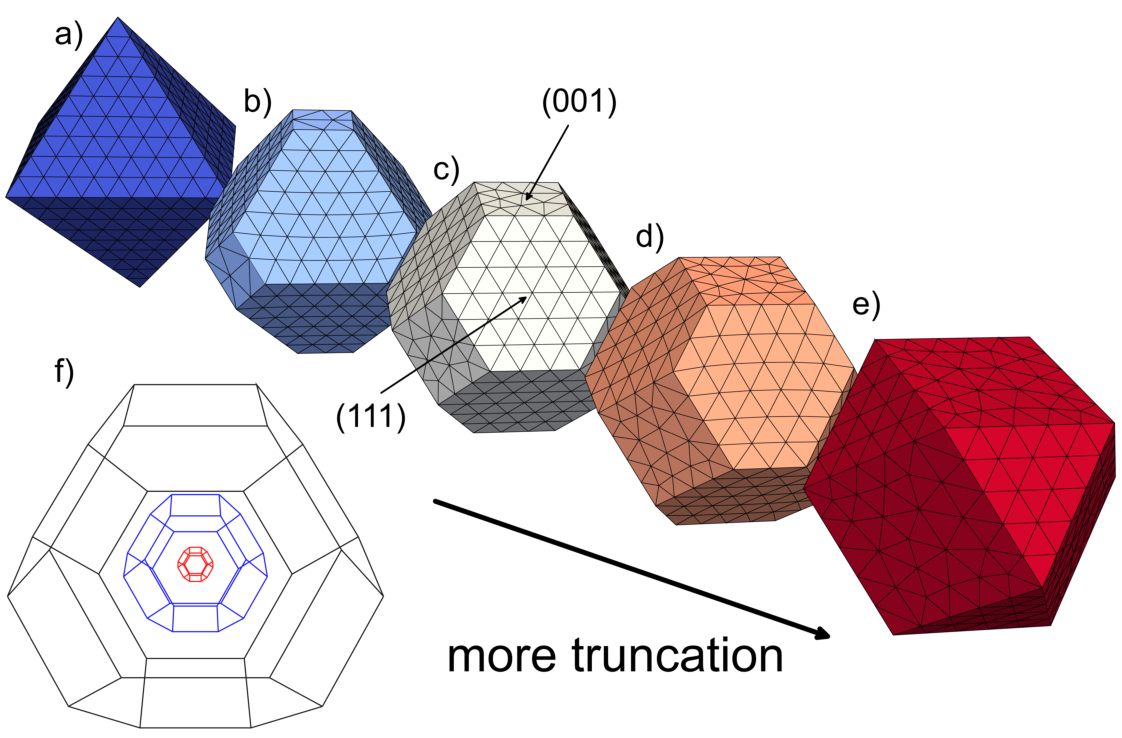
\includegraphics[width=\textwidth]{Figure_01_HR.pdf}
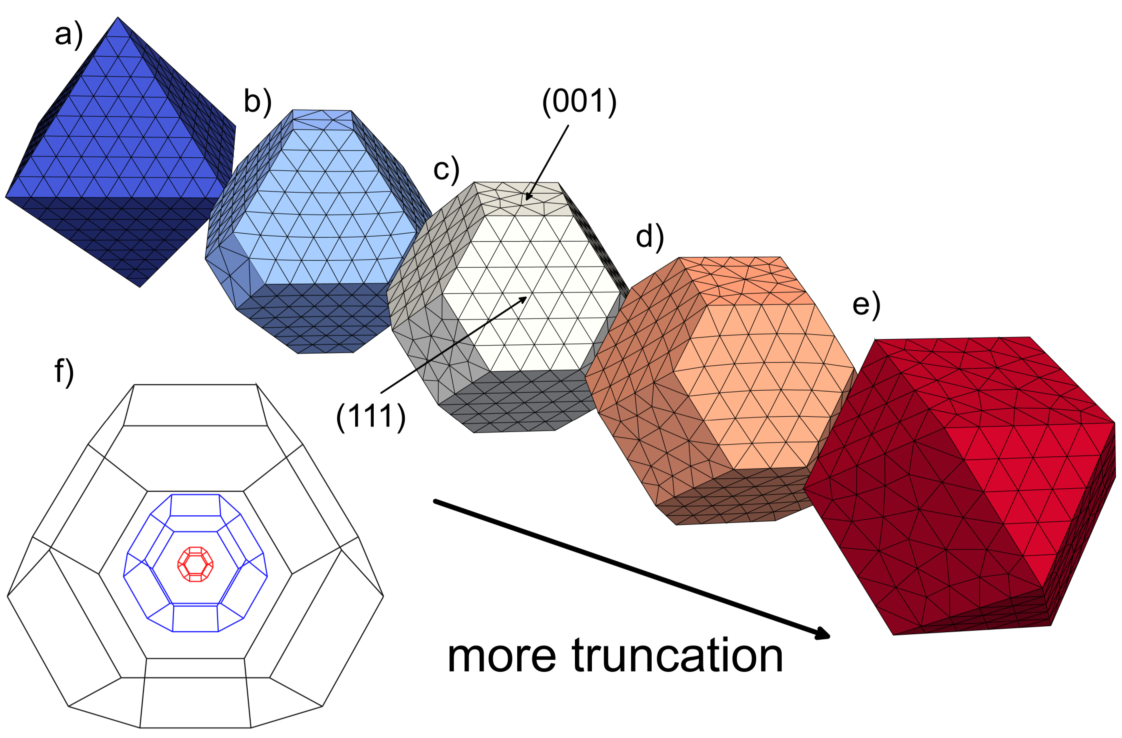
\includegraphics[width=\textwidth]{Figure_01.pdf}
\caption{FE meshes of the model euhedral geometries. From a) a regular octahedron, the rest are obtained by increasingly cutting more off the corners such that the edges of the octahedron are: b) halved (min. t. octahedron); c) reduced to a third (regular t. octahedron); d) reduced to a quarter (max. t. octahedron). e) A regular cuboctahedron is obtained by truncating to the point where the octahedron edges disappear entirely. The easy axes of magnetisation are the $<$111$>$ and the hard are the $<$001$>$, which are normal to the hexagonal $\{111\}$ and square $\{001\}$ faces, respectively, of the truncated octahedra. For a sense of scale, f) three nested regular truncated octahedra are shown with sizes 30$\,\text{nm}$ (red), 120$\,\text{nm}$ (blue) and 300$\,\text{nm}$ (black).}
\label{fig1}
\end{figure}


\end{document}